\subsection{Horizontal axis accuracy by the $d(K^-, (\Lambda \pi^-)_{CDS})"p"$ events}
\begin{figure}[htbp]
  \centering
  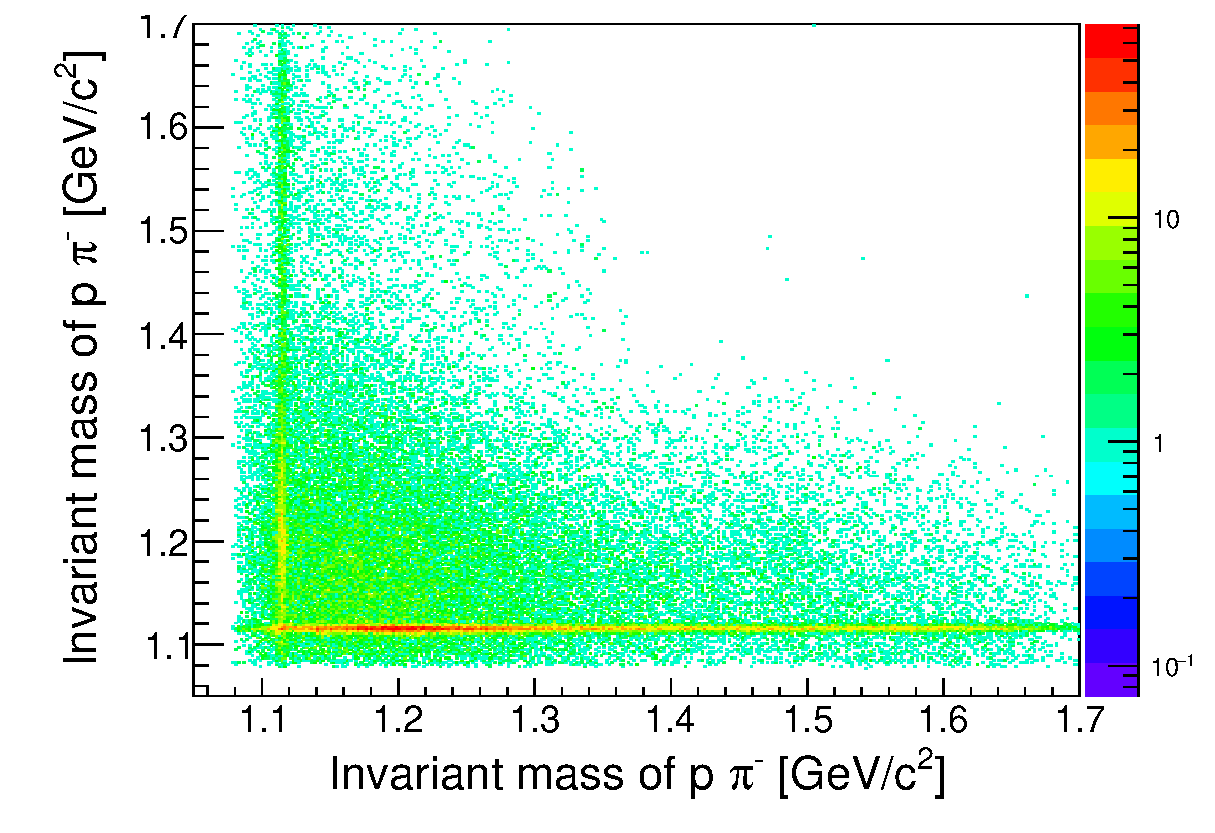
\includegraphics[width=8cm]{../pic/Dron/CDS_IM_ppim_p_2pim_2D.eps}
  \caption{
    This figures shows 2-D plot of $p$ $\pi^-$ invariant masses.
    The horizontal axis represents about near DCA pair and the vertical axis represents about the other pair.
  }
  \label{fig:CDS_2D_ppim_IM}
\end{figure}
\begin{figure}[htbp]
  \centering
  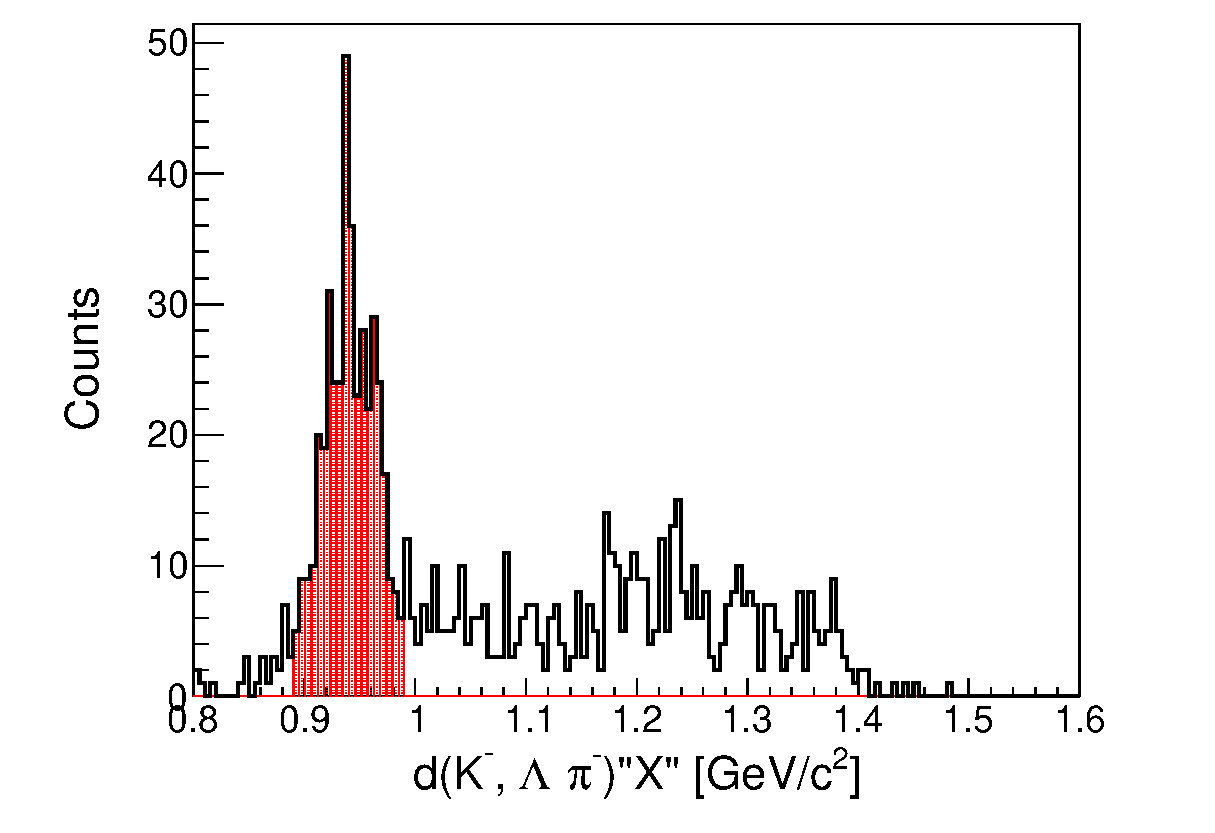
\includegraphics[width=8cm]{../pic/Dron/CDS_Lpim_MM_trigC.eps}
  \caption{
    This figure shows the missing mass of $d(K^-, \Lambda \pi^-)$ in events $\Lambda$ and $\pi^-$ was detected by the CDS.
    The red hatched region indicates the selection region as missing proton.
  }
  \label{fig:CDS_Lpim_MM}
\end{figure}

\begin{figure}
  \centering
  \begin{tabular}{cc}
    \begin{minipage}{0.5\hsize}
      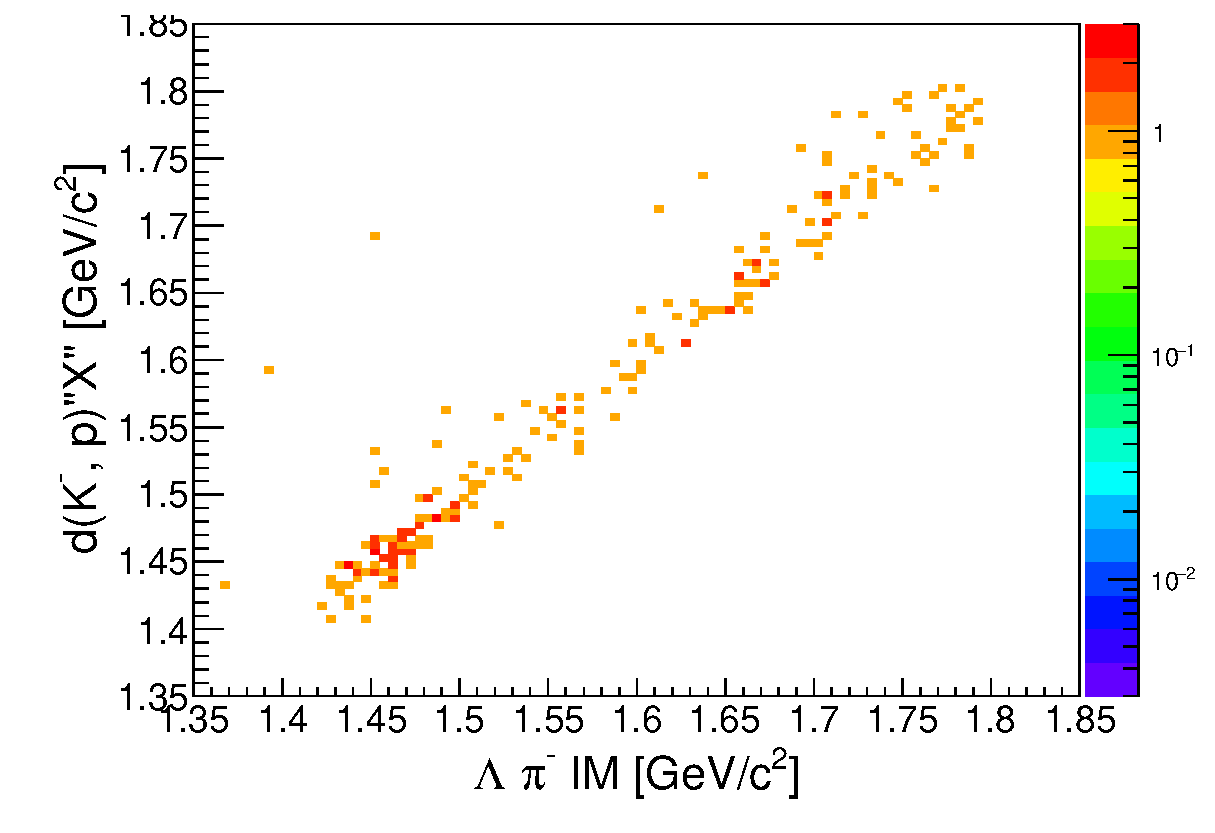
\includegraphics[width=7cm]{../pic/Dron/Lpim_IM_KP_MM.eps}
    \end{minipage}
    \begin{minipage}{0.5\hsize}
      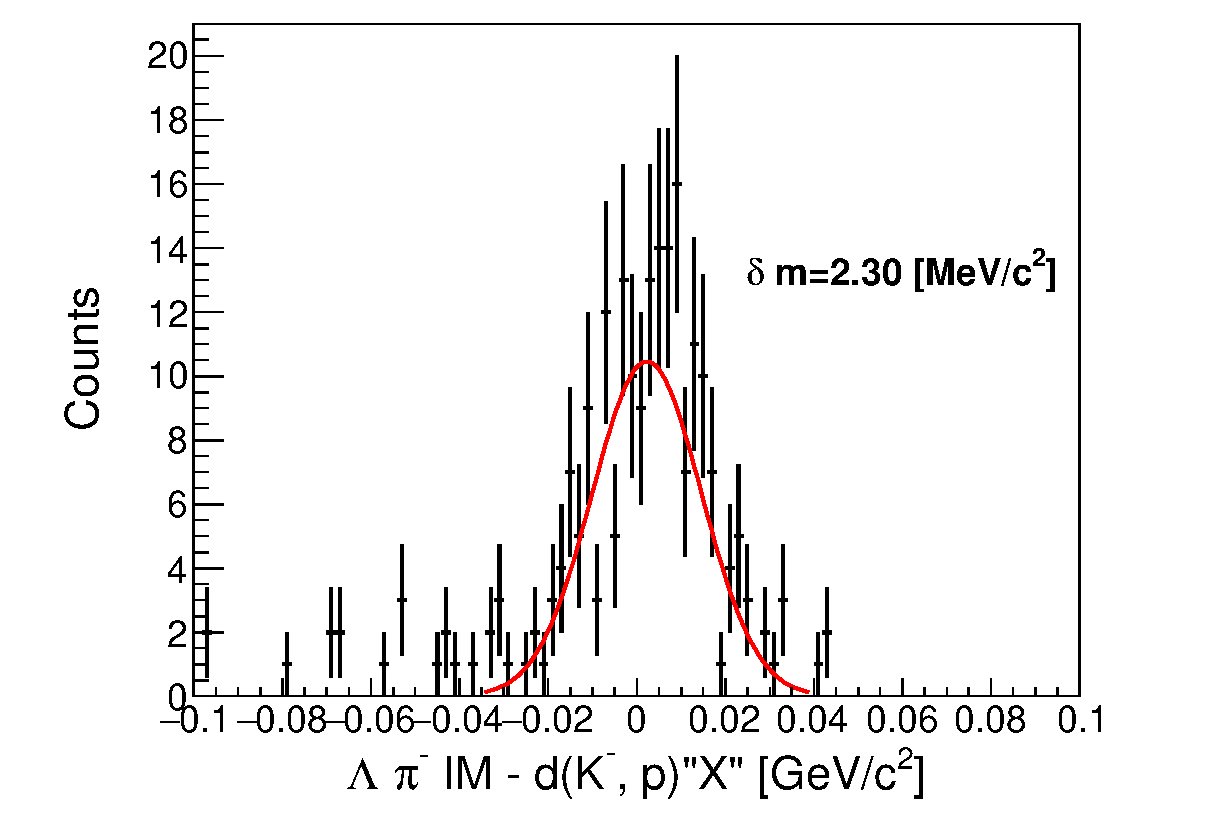
\includegraphics[width=7cm]{../pic/Dron/Lpim_IM_KP_MM_diff.eps}
    \end{minipage}
  \end{tabular}
  \caption{
    These figure indicate relation of $d(K^-, p)"X"$ and $\Lambda \pi^-$ invariant mass in events which detect $Lambda$ and $\pi^-$ by the CDS and $p$ by the PC/CVC.
    Left figure shows scatter plot and right figure represents subtraction distribution from invaraint mass to $d(K^-, p)"X"$.
  }
  \label{fig:CDS_Lpim_KP}
\end{figure}

The horizontal axis accuracy was also confirmed using the $K^- + d \rightarrow p + \Lambda + \pi$ reaction.
For this, the $d(K^-, (\Lambda \pi^-)_{CDS})"p"$ events were serached from events in which 2 $\pi^-$ and the proton were detected by the CDS.
And the $\Lambda$ reconstructed from the $\pi^-$ and the proton in these events which was shown as Fig\ref{fig:CDS_2D_ppim_IM}.
Next, the $d18k^-, \Lambda \pi^-)"p"$ events were identified as the Fig\ref{fig:CDS_Lpim_MM} which was indicated red plot.

Fig.\ref{fig:CDS_Lpim_KP} represents the correlation of the $Lambda \pi^-$ mass in events analyzing the forward proton additionally above contition.
In the left figure, the vertical axis indicates the $d(K^-, p)"\Lambda \pi^-"$ ant the horizontal axis indicates the invariant mass of the $\Lambda \pi^-$.
The right figure indicates the difference of these.
That indicates the accuracy of the missing mass of the d(K-, p) is about a few $MeV/c^2$.

% In events which detect two $\pi^-$ and proton by the CDS, $d(K^-, \Lambda \pi^-)"p"$ events  was observed.
% These events can be used to confirm accuracy of missing mass of $d(K^-, p)$.
% Fig\ref{fig:CDS_2D_ppim_IM} shows scatter plot invariant mass of $p$ $\pi^-$ which was observed $\Lambda$ locaus.
% The missng mass spectra of the $d(K^-, \Lambda \pi^-)"X"$ in forward charge trigger was represented in Fig\ref{fig:CDS_Lpim_MM}, which was clearly seen the $d(K^-, \Lambda \pi^-)"p"$ peak.

% Fig\ref{fig:CDS_Lpim_KP} represents relation of the $\Lambda \pi^-$ invariant mass and missing mass of the $d(K^-, p)"X"$.
% Difference of missing mass of the $d(K^-, p)"X"$ and invariant mass of the $\Lambda \pi^-$ was estimated at $2.3 MeV/c^2$.


